\section{Synthesis}
\label{sec:synthesis}

Given an SRE $A$ describing some property of a black-box system under
test, \autoref{theorem:sound} ensures that a well-typed test generator
program $\emptyset \vdash e : \uhat{\epsilon}{\Unit}{F}$ \emph{must}
be able to produce \emph{every} trace $\alpha$ that is consistent with
both $F$ and $A$, i.e. $\alpha \in F \land A$. Thus, the high-level
goal of our synthesis procedure is to find a generator that a) uses
effectful operators in a way that is consistent with the temporal and
data-dependency constraints captured by their specifications in
$\Delta$, and b) has a \tyName{} whose future automata shares a
meaningful overlap with $A$. Our synthesis algorithm simultaneously
solves both problems by using a loop, depicted in
\autoref{fig:syn-gen}, to iteratively \emph{refine} the target SRE
into a set of more concrete SREs, each of which can be directly mapped
to a well-typed generator program. Each iteration of this loop targets
a single event in an element of this set and adds events before and
after that event so that its dependences are satisfied, ensuring that
the corresponding operator in a synthesized program is well-typed. Our
loop also employs a regex non-emptiness check to ensure that each
element of the represents a generator that produces at least one
feasible trace. After the refinement loop has finished, a well-typed
generator programs can be mechanically extracted using the refined
property as a template.

\begin{figure}[h!]
  \vspace*{-.15in}
  \centering
  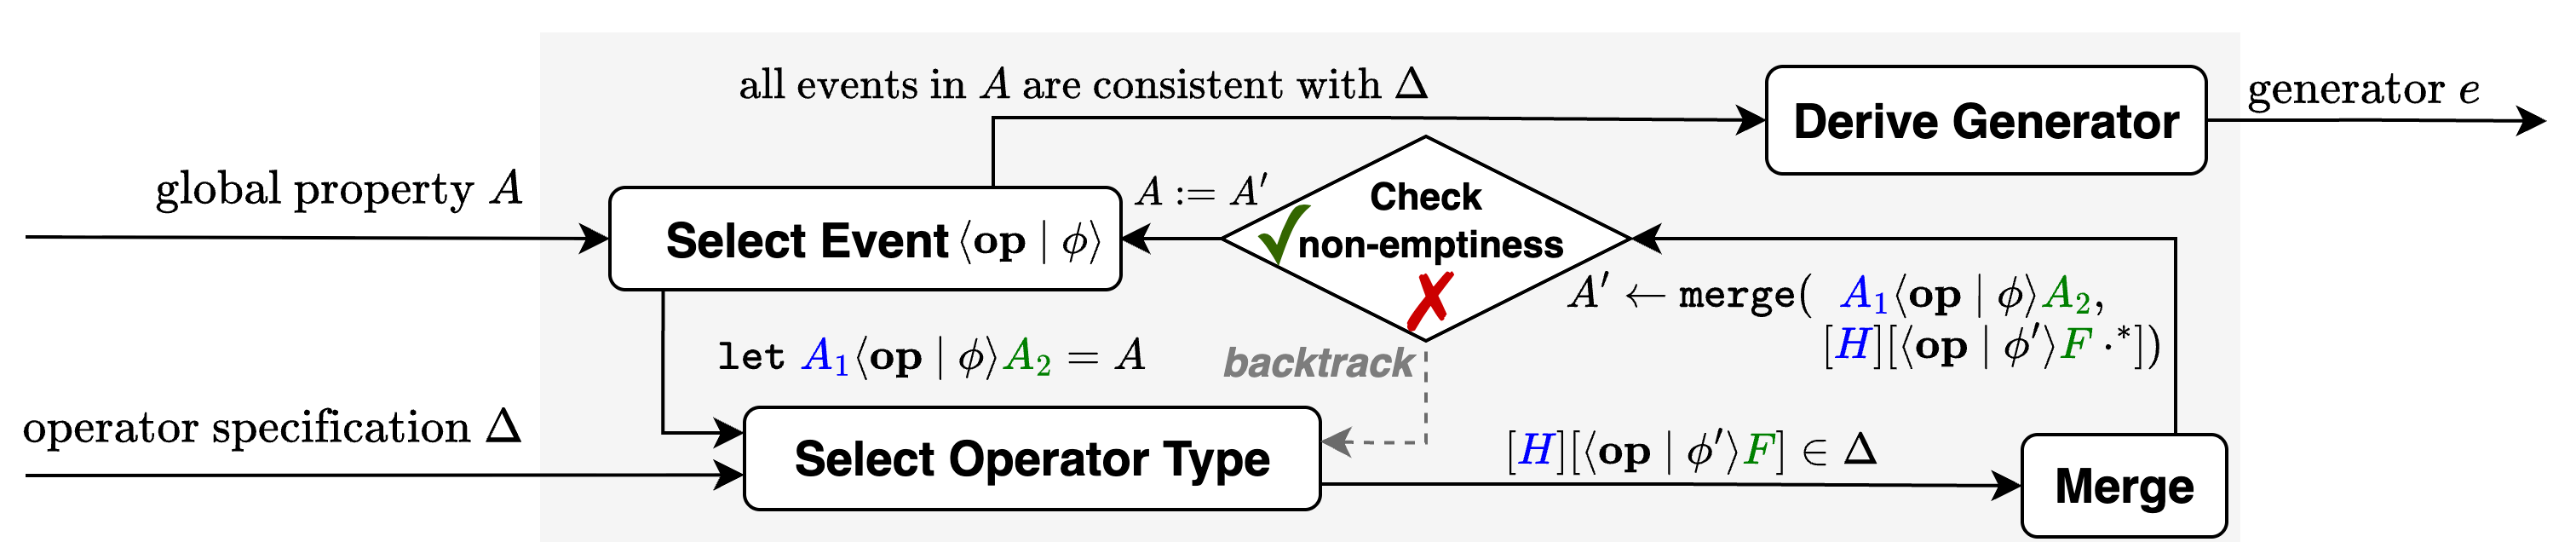
\includegraphics[width=0.75\linewidth]{figures/syn-gen.drawio.png}
  \caption{\name{}'s high-level test generator synthesis algorithm}
  \vspace*{-.15in}
  \label{fig:syn-gen}
  \vspace*{-.15in}
\end{figure}

\subsection{Synthesis Algorithm}

The main refinement loop in our synthesis algorithm operates over
\emph{abstract traces} --- sequences of symbolic events
$\msg{op}{\phi}$ plus alternatives defined by the following grammar: %
\vspace{-.4cm} \par\nobreak {\small
  \begin{flalign*}
    &\text{\textbf{Abstract Trace}} \quad \pi ::= \epsilon ~|~
    \msg{op}{\phi}^b ~|~ \pi \seqA \pi ~|~
    [\overline{\msg{op}{\phi}^b}]^*
  \end{flalign*}}\noindent Each symbolic event $\msg{op}{\phi}^b$ in
an abstract trace is tagged with a boolean $b$ indicating whether the
surrounding context satisfies its constraints. Operating over abstract
traces helps our synthesizer easily identify events with unresolved
dependencies. Every SRE can be normalized into a set of abstract
traces via an algorithm that applies a standard minimization algorithm
and then decomposes unions into abstract traces:
$\msg{op_1}{\phi_1} \cup \msg{op_2}{\phi_2}$ becomes
$\{\msg{op_1}{\phi_1}^\bot, \msg{op_2}{\phi_2}^\bot\}$, for
example.\footnote{The full definition of our SRE normalization
  procedure is provided in the \techreport{}.}

\begin{example}[SRE Normalization]\label{ex:sre-norm}
  The set of abstract traces corresponding to the history regex of
  $\eff{pop}$ from Example~\ref{ex:stack-example} includes the
  following abstract trace: %
  \vspace{-.4cm} \par\nobreak {\footnotesize %
    \begin{align*}
      \text{Original SRE:} \quad&  \Code{Last}(\msgAGray{popI}{m\;\_}) \land \Code{Last}(\msgAGray{pushI}{n\;\_}) \land (\allA\msgAGray{pushI}{(n{-}m)\;x}\allA)
      \\
      \text{One normalized trace:} \quad& \Pi_\Code{any}^*\seqA \msgAGray{popI}{m\;\_}^\bot \seqA \Pi_\Code{noPopI}^* \msgAGray{pushI}{(n-m)\;x}^\bot \seqA\Pi_\Code{noPopI}^* \msgAGray{pushI}{n\;\_}^\bot \seqA \Pi_\Code{noI}^* \tag{$\pi_\Code{pop1}$}\label{prop:popHis1}
      \\[-0.2em]
      \text{where} \quad& \Pi_\Code{any} \equiv [\msgCGray{pushI}^\bot \mid \msgCGray{popI}^\bot \mid \msgC{push}^\bot \mid \msgC{pop}^\bot]
      \\[-0.2em]
                                & \Pi_\Code{noPopI} \equiv [\msgCGray{pushI}^\bot \mid \msgC{push}^\bot \mid \msgC{pop}^\bot] \qquad\quad \Pi_\Code{noI} \equiv [\msgC{push}^\bot \mid \msgC{pop}^\bot]
    \end{align*}}\noindent
  This abstract trace imposes an ordering on the three intersected
  symbolic events in the original SRE; other traces correspond to
  different orderings. The alternatives after
  $\msgAGray{popI}{m\;\_}$ and $\msgAGray{pushI}{(n-m)\;x}$ in the
  trace disallow $\msgCGray{popI}$ event and
  $\msgCGray{pushI}$ events, respectively. The minimization step
  also produces traces that merge these intersected events: the
  procedure automatically considers the case where $m = 0$, which
  unifies the two $\effGray{pushI}$ events, resulting in the inclusion
  of the following abstract trace in the normalized set: %
  \vspace{-.4cm} \par\nobreak {\small %
\begin{align*}
  \Pi_\Code{any}^* \seqA \msgAGray{popI}{0\;\_}^\bot \seqA
  \Pi_\Code{noPopI}^* \seqA \msgAGray{pushI}{n\;x}^\bot \seqA \Pi_\Code{noI}^* \tag{$\pi_\Code{pop2}$}\label{prop:popHis2}
\end{align*}}\noindent
\end{example}

\setlength{\textfloatsep}{4pt}
\begin{algorithm}[t!]
  \Params{\quad Operator context $\Delta$, variables $\overline{x{:}b}$, and
    target trace property $A$}%
  \Output{\quad Generator $e$, such that
    $\overline{x{:}\urt{b}{\top}} \vdash e :
    \uhat{\epsilon}{\Unit}{A'} \land%
    \overline{x{:}\urt{b}{\top}} \vdash A' \subseteq A$} %
  $\Gamma \leftarrow \overline{x{:}\urt{b}{\top}}$ \tcp*[l]{initial
    type context} %
  $C \leftarrow \{(\Gamma, \pi) ~\mid~ \pi \in \normPlan(A)\}$
  \tcp*[l]{initialize set of abstract traces} %
  \While(\tcp*[h]{events still need to be refined}) %
  { %
    $\exists (\Gamma', \pi) \in C.\; %
    \pi = \pi_h \seqA \msg{op}{\phi}^\bot \seqA \pi_f$ } {
    $\Pi \leftarrow \refine(\Delta, \Gamma', \pi_h,
    \msg{op}{\phi}^\bot, \pi_f) \cup C - \{(\Gamma', \pi)\}$ }
\Return{$\derive(C)$} \tcp*[l]{synthesize recursions and derive generator program}
\caption{Test Generator Synthesis}
\label{algo:top-syn}
\end{algorithm}

\setlength{\textfloatsep}{4pt}
\begin{algorithm}[t!]
    \Params{\quad Operator context $\Delta$, typing context $\Gamma$,
      abstract trace $\pi_h \seqA \msg{op}{\phi}^\bot \seqA \pi_f$}%
    \Output{\quad Set of refined abstract traces $\Pi$ where the
      dependencies of $\msg{op}{\phi}$ are satisfied}
    $\overline{z{:}b}\garr\overline{y{:}t_y}\sarr\uhat{H}{x{:}t_x}{\msg{op}{\phi'}\seqA
      F} \leftarrow \Delta(\eff{op})$\tcp*[l]{retrieve \tyName of
      $\eff{op}$} %
    $\Gamma' \leftarrow \Gamma, \overline{z{:}\urt{b}{\top}},
    \overline{y{:}t_y}, x{:}t_x$ \tcp*[l]{add ghost variables and
      parameters types to type context} %
    $\msg{op}{\phi''} \leftarrow \msg{op}{\phi \land \phi'}$
    \tcp*[l]{refine target operation} %
    $H' \leftarrow \pi_h \land H$ \tcp*[l]{merge history regex}
    $F' \leftarrow \pi_f \land (F \seqA \allA)$ \tcp*[l]{merge future
      regex} %
    $ P \leftarrow \normPlan(H'\seqA \msg{op}{\phi''}^\top\seqA F')$
    \tcp*[l]{normalize refined trace} %
    \Return{$\{(\Gamma', \pi') \mid \pi' \in P \land \Gamma' \vdash
      \pi' \not \subseteq \emptyset \}$}
    \tcp*[l]{filter empty abstract traces} %
    \caption{Abstract Trace Refinement (\refine{})}
\label{algo:refine}
\end{algorithm}

Our top-level synthesis algorithm is shown in \autoref{algo:top-syn}.
Given a target trace property $A$ whose qualifiers only contain the
variables $\overline{x{:}b}$, this algorithm synthesizes a well-typed
$\DSL{}$ generator. The algorithm maintains a set of candidate
abstract traces, $C$, each of which is a refinement of $A$; this set
is initialized directly from $A$ (line 2). Each trace in $C$ is paired
with a typing context that the synthesizer uses to filter out
refinements that do not correspond to well-typed programs. The
algorithm first uses a loop (lines $3-4$) to refine $C$ until it only
contains abstract traces that are consistent with the operator context
$\Delta$, and then uses the resulting set of traces to derive the
final (recursive) generator (line $5$). Each iteration of this loop
nondeterministically chooses a target event in one of the current
abstract traces (line $2$) whose tag indicates its dependencies are
not satisfied; it then uses the $\refine$ subroutine to insert the
required operations before and after the target event.

\paragraph{Abstract trace refinement} The abstract trace refinement
subroutine, \refine{}, is shown in \autoref{algo:refine}. It first
retrieves the \tyName{} of the target operation $\eff{op}$ from
$\Delta$ (line $1$), and adds its parameters to the type context (line
$3$). \refine{} then merges the selected \tyName{} with the current
abstract trace (lines $4-6$) and normalizes the result to produce a
set of refinements of the input trace that are consistent with
$\eff{op}$ (line $7$).  Line $6$ effectively applies the
\textsc{SubHF} rule to drop any states that are unreachable after the
target operation; while line 4 effectively applies \textsc{TOpHis} to
ensure the trace that precedes the target operation satisfies its
specification. % \BD{The careful reader will notice we're using a very
  % precise specification of an operator here... Do we need to argue why
  % that's okay?}
Before returning the refined trace, \refine{} checks that it
corresponds to a meaningful test generator by filtering out any empty
traces (line $7$).

\begin{example}[Abstract Trace Refinement]\label{ex:refinement-process}
  We illustrate the refinement process by showing how it derives a
  trace corresponding to the generator from in
  Example~\ref{ex:operator-application-typing}. Assume the refinement
  loop begins with the following (singleton) set of abstract traces:
  \vspace{-.4cm} \par\nobreak {\small %
    \begin{align*}
      \Pi_\Code{any}^* \seqA \msg{pop}{\top} \seqA \Pi_\Code{any}^*
    \end{align*}}\noindent
  where the user requires that the test generator performs at least
  one $\eff{pop}$ operation.  In the first iteration, the symbolic
  event $\msg{pop}{\top}$ is selected for refinement using
  \refine{}. The algorithm first retrieves the \tyName{} of
  $\eff{pop}$ from $\Delta$: %
  \vspace{-.4cm} \par\nobreak{\small %
    \begin{align*}
      &\Delta(\eff{pop}) \equiv
        n{:}\Int \garr m{:}\Int \garr \uhat{\pi_\Code{pop1} \cup \pi_\Code{pop2} \cup ...}{x{:}\Int}{\msgA{pop}{x}\seqA\msgAGray{popI}{m{+}1\;x}}\seqA\Pi_\Code{any}^*
    \end{align*}}%
  \noindent We have normalized the history regex to illustrate that
  merging this \tyName{} with the current abstract trace and
  normalizing can result in multiple new abstract traces.  For
  example, property~\ref{prop:popHis2} in the history regex can yield
  the following trace: %
  \vspace{-.4cm} \par\nobreak{\small %
  \begin{align*}
    &(m{:}\urt{\Int}{\vnu = 0}, n{:}\urt{\Int}{\top},y{:}\urt{\Int}{\top},x{:}\urt{\Int}{\top}, \\
    &\qquad\qquad \Pi_\Code{any}^* \msgAGray{popI}{m\;y}^\bot \Pi_\Code{noPopI}^* \msgAGray{pushI}{n\;x}^\bot \Pi_\Code{noI}^* \msgA{pop}{x}^\top\msgAGray{popI}{m\;x}^\bot)
  \end{align*}} \vspace{-.4cm} \par\nobreak\noindent
The new variables in the type context require $m = 0$, as
mentioned in Example~\ref{ex:sre-norm}.  Although the \tyName{} of
$\eff{pop}$ does not explicitly add any new $\eff{push}$ or
$\eff{pop}$ events to the abstract trace, it does require multiple
ghost events, which will recover corresponding concrete events during
further refinement.  For example, the \tyName{} of $\effGray{pushI}$
is given below; it requires that a $\eff{pushI}$ event always occurs
after a $\eff{push}$ event, unless it is an initialization event
(i.e., $i = 0$): %
\vspace{-.4cm} \par\nobreak{\footnotesize %
  \begin{align*}
    \Delta(\effGray{pushI}) \equiv &\; i{:}\Int\sarr x{:}\Int \sarr \uhat{\allA\msgC{push}}{\Unit}{\msgBGray{pushI}{i\;x}{i > 0}} \interty \uhat{(\anyA\setminus\msgCGray{pushI})^*}{\Unit}{\msgBGray{pushI}{i\;x}{i = 0}} \\
    \Delta(\effGray{popI}) \equiv &\; i{:}\Int\sarr x{:}\Int \sarr \uhat{\allA\msgC{pop}}{\Unit}{\msgBGray{popI}{i\;x}{i > 0}} \interty \uhat{(\anyA\setminus\msgCGray{popI})^*}{\Unit}{\msgBGray{popI}{i\;x}{i = 0}}
  \end{align*}}\vspace{-.4cm} \par\nobreak\noindent
On the other hand, the $\msgAGray{popI}{m\;y}$ event in the abstract trace has index $m = 0$, and the algorithm can smartly determine that there is no previous $\eff{pop}$ event in this case. It is because the merge result of the first intersected type of $\effGray{popI}$ fails the non-emptiness check, where $m > 0 \land m = 0$ is unsatisfiable. Finally, this trace will be refined to one consistent with the program shown in Example~\ref{ex:operator-application-typing}:
\vspace{-.4cm} \par\nobreak{\small %
  \begin{align*}
    &(m{:}\urt{\Int}{\vnu = 0}, n{:}\urt{\Int}{\vnu = m{+}1}, y{:}\urt{\Int}{\top}, x{:}\urt{\Int}{\vnu > y},
    \\&\qquad\qquad\Pi_\Code{noI}^* \seqA \msgAGray{pushI}{m\;y}^\bot
    \seqA \msgAGray{popI}{m\;y}^\bot \seqA \Pi_\Code{noI}^* \seqA \msgA{push}{x}^\bot \seqA \msgAGray{pushI}{n\;x}^\bot \seqA \Pi_\Code{noI}^* \seqA \msgA{pop}{x}^\top \seqA \msgAGray{popI}{n\;x}^\bot \seqA \Pi_\Code{any}^*) \tag{$\pi_\Code{stack}$}\label{prop:stackTrace}
  \end{align*}}\vspace{-.4cm} \par\nobreak\noindent
\end{example}

\paragraph{Deriving a Generator}
The second component of our synthesis algorithm, \derive{}, derives
generators for each abstract trace in the set produced the refinement
loop and then combines them using $\oplus$ to construct the final
generator.  This process relies on a subroutine, \deriveTrace{}, that
generates straightline programs without recursion by dropping by all
ghost events and variables and then mapping each symbolic event to a
corresponding effectful operation with appropriate arguments. So,
given the following context and abstract trace:
\vspace{-.4cm} \par\nobreak{\small%
  \begin{align*} (m{:}\urt{\Int}{\vnu = 0}, n{:}\urt{\Int}{\vnu =
      m{+}1}, y{:}\urt{\Int}{\top}, x{:}\urt{\Int}{\vnu > y},
    \msgA{push}{x} \seqA \msgA{pop}{x})
  \end{align*}
}\noindent \deriveTrace{} will synthesize the following program:
\begin{minted}[fontsize = \footnotesize, escapeinside=??, xleftmargin=10pt, linenos]{ocaml}
  let (x: int) = ?$\mykw{assume}\; (\exists m\;n\;y. m = 0 \land n = m{+}1 \land x > y)$? in push x; (* equivalent to assume true *)
  let (z: int) = pop () in assert (x == z)
\end{minted}
\derive{} applies a sketch-style methodology to synthesize a recursive
generator, using \deriveTrace{} to fill in the holes of a template
recursive function definition. It does so by associating each of the
holes in the template with a subsequence of the abstract trace,
treating each occurence of a Kleene star in an abstract trace as a
candidate placeholder for a recursive call. In order to ensure a
particular partitioning is sensible, the algorithm simulates a bounded
number of loop iterations to ensure a completed sketch is well-typed.

% in abstract traces are interpreted as recursion
% points. The synthesis algorithm $\derive$ non-deterministically either
% (i) generates a sequential program by eliminating all ghost events and
% the Kleene stars \footnote{The definition of $\derive$ is provided in
%   the \techreport{}.}, or (ii) synthesizes a recursive program by
% expanding the Kleene star using recursion. We employ a template-based
% strategy, in which the algorithm matches the given abstract trace with a
% template $T$, together with abstract traces for the recursion body
% ($\Pi_{\Code{rec}}$), as well as its associated history ($\Pi_h$) and
% future ($\Pi_f$) traces. As dictated by \textsc{TFixInd}, the algorithm
% unrolls the recursive body up to a bounded depth and invokes
% refinement loop (lines 2-3 in \autoref{algo:top-syn}) to ensure that
% the unrolled abstract traces are well-typed. The synthesized programs
% for these three traces are then composed to instantiate the
% placeholders in the recursive template.

\begin{example}[Recursion Template]
  Consider the following template which defines and uses a recursive
  function $f$ that calls itself once:
  $T \doteq \zlet{f}{\mykw{fix}\ f.\lambda ().\ () \oplus \boxed{e_1};
    f\;(); \boxed{e_2}}{(\boxed{e_3};f\;();\boxed{e_4})}$. This
  template includes a pair of holes before and after the recursive
  call in the definition of $f$, and another pair around the top-level
  call to $f$. We can build the following two program sketches by
  mapping portions of $\pi_\Code{stack}$ from
  Example~\ref{ex:refinement-process} to the four holes in $T$: %
  \vspace{-.4cm} \par\nobreak {\footnotesize %
    \begin{align*}
      &
        \underbrace{\Pi_\Code{noI}^*\msgAGray{pushI}{m\;y}\msgAGray{popI}{m\;y}\Pi_\Code{noI}^*}_{e_3}\;\;
        \underbrace{\msgA{push}{x}\msgAGray{pushI}{n\;x}}_{e_1}\;\;
        \underbrace{\Pi_\Code{noI}^*}_\text{$f$\;()}\;\;
        \underbrace{\msgA{pop}{x}\msgAGray{popI}{n\;x}}_{e_2}\;\;
        \underbrace{\Pi_\Code{noI}^*}_{e_4}
      \\[5pt]
      & \underbrace{\Pi_\Code{noI}^*\msgAGray{pushI}{m\;y}\msgAGray{popI}{m\;y}\Pi_\Code{noI}^*\msgA{push}{x}\msgAGray{pushI}{n\;x}}_{e_3}\;\;
        \underbrace{\Pi_\Code{noI}^*}_{e_1}\;\;
        \underbrace{\Pi_\Code{noI}^*}_\text{$f$\;()}\;\;
        \underbrace{\msgA{pop}{x}\msgAGray{popI}{n\;x}}_{e_2}\;\;
        \underbrace{\Pi_\Code{noI}^*}_{e_4}
    \end{align*}}\vspace{-.4cm} \par\nobreak \noindent %
  We can then simulate unrolling the recursive call in a solution to
  each sketch by duplicating the subtraces labeled $e_1\; f\;()\;
  e_2$ a bounded number of times and checking whether they are consistent with
  $\pi_\Code{stack}$: doing so reveals that the second sketch would
  not yield a valid solution, as the recursive call would repeatedly
  perform $\eff{pop}$ events without any $\eff{push}$ events. The
  first sketch, in contrast, is consistent with $\pi_\Code{stack}$;
  using \deriveTrace{} to synthesize generators for each $e$ yields
  the following generator:
  \begin{minted}[fontsize = \footnotesize, escapeinside=??, xleftmargin=10pt, linenos]{ocaml}
let rec f () = () ?$\oplus$?
    let (x: int) = int_gen () in push x; (* ?$e_1$? *)
    f ();
    let (z: int) = pop () in assert (x == z) (* ?$e_2$? *)
in (* ?$e_3$? *) f () (* ?$e_4$? *)
  \end{minted}
\end{example}

\begin{theorem}[\autoref{algo:top-syn} is Sound]
  \label{theorem:algo-sound}
  Every generator synthesized by \autoref{algo:top-syn} is type-safe
  with respect to our declarative typing system.
\end{theorem}
